\section{Introduzione}\label{sec:introduzione}

\subsection{Scopo del Documento}\label{sec:scopo_del_documento}
Il presente documento ha lo scopo di fornire una descrizione dettagliata dei requisiti di progetto. Il documento é quindi frutto di un'attenta analisi del capitolato, proposto dal proponente, al fine di individuare ed esaminare in modo esaustivo i requisiti minimi, massimi e facoltativi presenti nel progetto. 
Un ulteriore obbiettivo del documento é quello di analizzare e descrivere le possibili attività (use cases) permesse all'utente in fase di esecuzione del programma. 

\subsection{Glossario}\label{sec:glossario}

Al fine di evitare incomprensioni relative alla terminologia usata all’interno del presente documento, viene 
fornito un Glossario di progetto. Ogni terminologia specifica di progetto verrà chiarita e definita in modo tale 
da renderla maggiornamente comprensibile ed evitare errate interpretazioni. Pertanto ogni termine marchiato
con una lettera G come apice, sarà specificato e presente nel glossario sopra citato.

\subsection{Riferimenti}\label{sec:riferimenti}

\subsubsection{Riferimenti normativi}\label{sec:riferimenti_normativi}
\begin{itemize}
    \item Norme di Progetto v1.0.0 \\
    ++++Inserire link alle norme di progetto++++
    \item Capitolato C5 - WMS3: wharehouse management 3D \\
    https://www.math.unipd.it/~tullio/IS-1/2023/Progetto/C5.pdf
\end{itemize}

\subsubsection{Riferimenti informativi}\label{sec:riferimenti_informativi}
\begin{itemize}
    \item Analisi e descrizione delle funzionalita: Use case e relativi diagrammi (UML) - materiale didattico corso
    di Ingegneria del Software\\
    https://www.math.unipd.it/rcardin/swea/2022/Diagrammi%20Use%20Case.pdf
    \item Analisi dei requisiti (T5) - materiale didattico corso di Ingegneria del Software\\
    https://www.math.unipd.it/~tullio/IS-1/2023/Dispense/T5.pdf
\end{itemize}

\newpage

\section{Descrizione}\label{sec:descrizione}

\subsection{Scopo del progetto}\label{sec:scopo_del_progetto}
Lo scopo del progetto é quello di ottimizzare i processi produttivi attraverso l'utilizzo di 
un applicativo 3D che rappresenta lo stato di fatto di un magazzino di stoccaggio.\\
L'applicativo, pensato per un'utilizzo da ufficio, deve permettere all'utente di navigare\textsuperscript{G} all'interno 
del magazzino e poter gestire le seguenti operazioni:
\begin{itemize}
    \item Creazione magazzino:
        \begin{itemize}
            \item Creare un nuovo magazzino
            \item Importare un layout esistente
        \end{itemize}
    \item Modifiche alla struttura del magazzino:
        \begin{itemize}
            \item Modificare scaffalature
            \item Aggiungere nuove scaffalature
            \item Rimuovere scaffalature esistenti
        \end{itemize}
    \item Modifiche ai prodotti presenti in magazzino:
        \begin{itemize}
            \item Eliminare un prodotto
            \item Aggiungere un nuovo prodotto
            \item Spostare un prodotto esistente 
        \end{itemize}
\end{itemize}
Sfruttare quindi un'esperienza tridimensionale per aiutare la comprensione e facilitare la gestione delle 
operazioni di logistica necessarie. 


\subsection{Descrizione del prodotto}\label{sec:descrizione_del_prodotto}

+++++ ancora da definire correttamente
L'applicativo, pensato per soddisfare lo scopo e i requisiti di progetto, si compone principalmente di due 
sezioni distinte. La prima sezione é composta dal terminale, attraverso il quale l'utente potrà interagire 
in modalità assistita\textsuperscript{G}. All'utente sarà infatti permesso, attraverso tale terminale, un certo numero di 
operazioni 
La seconda parte invece è composta dalla visualizzazione vera e proprio del magazzino 3D. In questa area 
l'utente avrà modo di "navigare" e 

\newpage

\section{Use Cases}\label{sec:use_cases}

\Large\textbf{}\\
\Large\textbf{Use Case X Creazione nuovo layout} \\
\vspace{0.5cm}
%\begin{figure}[h]
%  \centering
%  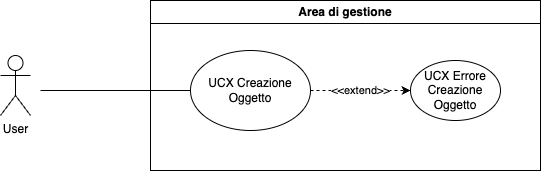
\includegraphics[width=0.8\textwidth]{UseCasesImages/ObjCr.png}
%\end{figure}

\large\textbf{} \\
\textbf{Attori:} User\\
\textbf{Pre-condizione:} Avvio dell'applicazione da parte dell'utente\\
\textbf{Post-condizione: } Creazione del layout magazzino\\
\textbf{Scenario Principale:}  All'utente viene richiesto se caricare un layout esistente o se creare da 0 il layout del magazzino.\\

\vspace{0.5cm}

\Large\textbf{}\\
\Large\textbf{Use Case X Creazione Nuovo magazzino} \\
\vspace{0.5cm}
%\begin{figure}[h]
%  \centering
%  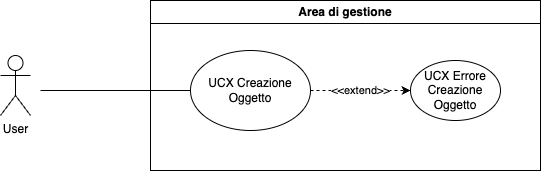
\includegraphics[width=0.8\textwidth]{UseCasesImages/ObjCr.png}
%\end{figure}

\large\textbf{} \\
\textbf{Attori:} User\\
\textbf{Pre-condizione:} E' stato selezionata la modalità: "creazione manuale magazzino" \\
\textbf{Post-condizione: } Creazione del nuovo layout del magazzino\\
\textbf{Scenario Principale:}  L'utente crea un nuovo layout magazzino inserendo le specifiche all'interno di un form prestabilito.\\
\textbf{Estensioni: } UCX Errore Creazione Layout magazzino\\

\vspace{0.5cm}

\textbf{}\\
{\color{red}{\textbf{Domanda:} Il magazzino può avere delle misure arbitrarie? Esistono dei massimi o dei minimi? }} \\
{\color{red}{\textbf{Domanda:} Il magazzino può essere suddiviso in sottoparti? Eventualmente queste sottoparti devono avere delle limitazioni fisiche (muri) o solamente ipotetiche (virtuali)?}}\\

\vspace{0.5cm}

\Large\textbf{}\\
\Large\textbf{Use Case X Importazione layout magazzino} \\
\vspace{0.5cm}
%\begin{figure}[h]
%  \centering
%  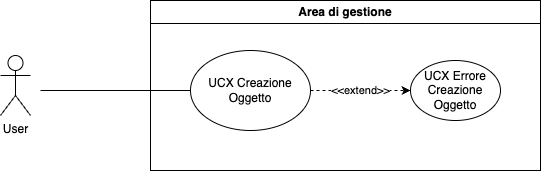
\includegraphics[width=0.8\textwidth]{UseCasesImages/ObjCr.png}
%\end{figure}

\large\textbf{} \\
\textbf{Attori:} User\\
\textbf{Pre-condizione:} E' stato selezionata la modalità: "importazione layout magazzino" \\
\textbf{Post-condizione: } Importazione Layout Magazzino\\
\textbf{Scenario Principale:}  Il magazzino viene correttamente importato da layout esistente.\\
\textbf{Estensioni: } UCX Errore Importazione Layout\\

\vspace{0.5cm}


\Large\textbf{}\\
\Large\textbf{Use Case X Creazione scaffalatura} \\
\vspace{0.5cm}
%\begin{figure}[h]
%  \centering
%  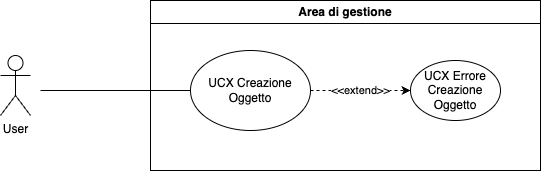
\includegraphics[width=0.8\textwidth]{UseCasesImages/ObjCr.png}
%\end{figure}

\large\textbf{} \\
\textbf{Attori:} User\\
\textbf{Pre-condizione:} Richiesta nuovi inserimento scaffalatura \\
\textbf{Post-condizione: } Creazione corretta della scaffalatura\\
\textbf{Scenario Principale:}  L'utente crea una nuova scaffalatura inserendone le \textit{specifiche caratteristiche}. Se i dati inseriti non rispettano il \textit{criterio prestabilito} viene visualizzato un messaggio di errore.\\
\textbf{Estensioni: } UCX Errore Creazione scaffalatura\\

\vspace{0.5cm}

\textbf{}\\
{\color{red}{\textbf{Domanda:} Una scaffalatura ha delle dimensioni standard o massime? Quanto e se è personalizzabile (sia per le dimensioni effettive della scaffalatura sia per le dimensioni interne degli spazi utili della scaffalatura)? }} \\
{\color{red}{\textbf{Domanda:} Abbiamo delle prescizioni particolari da rispettare? (Come per esempio lo spazio tra una scaffallatura e l'altra; il fatto di poterle "appoggiare una con l'altra") }}\\

\vspace{0.5cm}

\Large\textbf{}\\
\Large\textbf{Use Case X Spostamento scaffalatura} \\
\vspace{0.5cm}
%\begin{figure}[h]
%  \centering
%  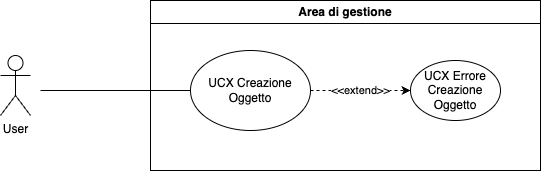
\includegraphics[width=0.8\textwidth]{UseCasesImages/ObjCr.png}
%\end{figure}

\large\textbf{} \\
\textbf{Attori:} User\\
\textbf{Pre-condizione:} Richiesta spostamento scaffalatura \\
\textbf{Post-condizione: } Scaffallatura spostata \\
\textbf{Scenario Principale:}  L'utente selezione la scaffalatura da spostare e il nuovo spazio dove posizionarla.\\
\textbf{Estensioni: } UCX Errore Spostamento Scaffallatura\\

\vspace{0.5cm}

\textbf{}\\
{\color{red}{\textbf{Domanda:} E' uno use case rilevante in termini pratici? E' da implementare? }} \\
{\color{red}{\textbf{Domanda:} Si era pensato di permettere lo spostamento solo a scaffaatura vuota, può essere corretto in termini pratici? }}\\

\vspace{0.5cm}

\Large\textbf{}\\
\Large\textbf{Use Case X Modifica scaffalatura} \\
\vspace{0.5cm}
%\begin{figure}[h]
%  \centering
%  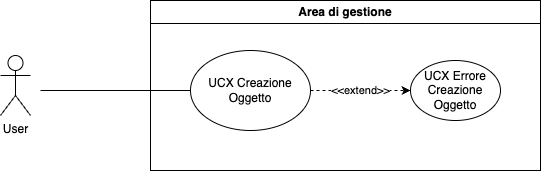
\includegraphics[width=0.8\textwidth]{UseCasesImages/ObjCr.png}
%\end{figure}

\large\textbf{} \\
\textbf{Attori:} User\\
\textbf{Pre-condizione:} Scaffallatura correttamente presente \\
\textbf{Post-condizione: } Corretta modifica scaffalatura\\
\textbf{Scenario Principale:}  L'utente modifica la scaffalatura esistente. \\
\textbf{Estensioni: } UCX Errore modifica scaffalatura\\

\vspace{0.5cm}

\textbf{}\\
{\color{red}{\textbf{Domanda:} Anche in questo caso è possibile modificare solamente la struttura "esterna" della scaffaatura oppure anche gli "spazi interni"? Abbiamo qualche vincolo particolare da rispettare? }} \\

\vspace{0.5cm}
\Large\textbf{}\\
\Large\textbf{Use Case X Creazione Oggetto} \\
\vspace{0.5cm}
%\begin{figure}[h]
%  \centering
%  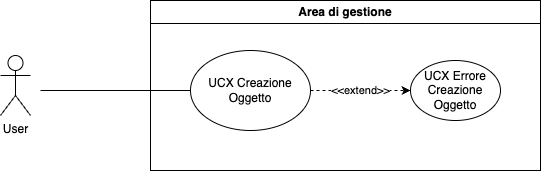
\includegraphics[width=0.8\textwidth]{UseCasesImages/ObjCr.png}
%\end{figure}

\large\textbf{} \\
\textbf{Attori:} User\\
\textbf{Pre-condizione:} Magazzino correttamente istanziato \\
\textbf{Post-condizione: } Creazione Oggetto\\
\textbf{Scenario Principale:}  L'utente crea un oggetto inserendone le \textit{specifiche caratteristiche}. Se i dati inseriti non rispettano il \textit{criterio prestabilito} viene visualizzato un messaggio di errore.\\
\textbf{Estensioni: } UCX Errore Creazione Oggetto\\

\vspace{0.5cm}

\textbf{}\\
{\color{red}{\textbf{Domanda:} Un oggetto puó essere creato e memorizzato in uno spazio apposito senza essere inserito in una scaffalatura o la creazione coincide con l'inserimento?}} \\
{\color{red}{\textbf{Domanda:} Quali sono le caratteristiche di un oggetto? In particolare: \\-Un oggetto puó superare i limiti di dimensione di una scaffalatura? \\ -Gli oggetti hanno forma standardizzata?}}\\

\vspace{0.5cm}

\Large\textbf{}\\
\Large\textbf{Use Case X Errore Creazione Oggetto} \\
\large\textbf{} \\
\textbf{Attori:} User\\
\textbf{Pre-condizione:} L'utente ha inserito dati scorretti nella schermata di creazione di un oggetto\\
\textbf{Post-condizione: } Visualizzazione Errore\\
\textbf{Scenario Principale:} Il sistema mostra a schermo un messaggio contenente le specifiche dell'errore di inserimento\\

\vspace{0.5cm}

\Large\textbf{}\\
\Large\textbf{Use Case X Ricerca Statica Oggetto} \\
\vspace{0.5cm}
%\begin{figure}[h]
%  \centering
%  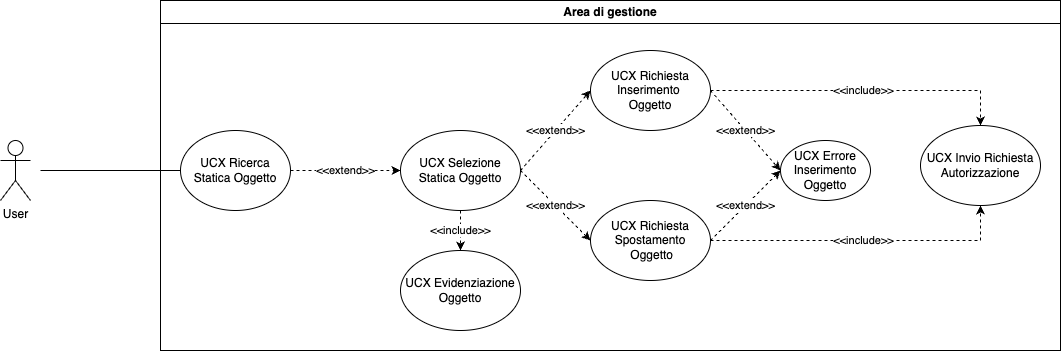
\includegraphics[width=0.8\textwidth]{UseCasesImages/StaticRes.png}
%\end{figure}

\large\textbf{} \\
\textbf{Attori:} User\\
\textbf{Pre-condizione:} Magazzino correttamente istanziato, l'user si ritrova nell'area di gestione \\
\textbf{Post-condizione: } Visualizzazione lista oggetti corrispondenti a dati inseriti\\
\textbf{Scenario Principale:}  L'utente effettua una ricerca seguendo dei particolari \textit{parametri} e il sistema ritorna una lista (anche vuota) di oggetti corrispondenti. Sará poi possibile selezionare gli oggetti\\
\textbf{Estensione:} UCX Selezione Statica Oggetto

\textbf{}\\
{\color{red}{\textbf{Domanda:} Quali sono i parametri di ricerca degli oggetti?}}\\

\vspace{0.5cm}

\Large\textbf{}\\
\Large\textbf{Use Case X Selezione Statica Oggetto} \\
%\begin{figure}[h]
%  \centering
%  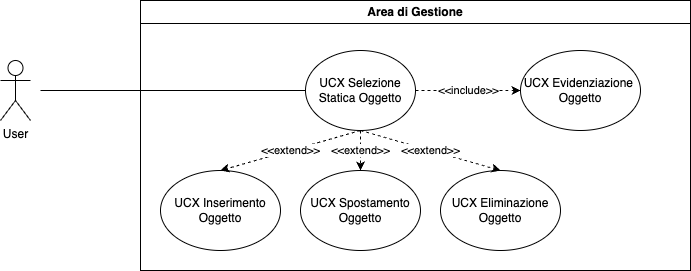
\includegraphics[width=0.8\textwidth]{UseCasesImages/StaticSel.png}
%\end{figure}

\vspace{0.5cm}

\large\textbf{} \\
\textbf{Attori:} User\\
\textbf{Pre-condizione:} L'user si trova nell'area di gestione e sta visualizzando una lista di oggetti \\
\textbf{Post-condizione: } Selezione di un oggetto e relativa evidenziazione\\
\textbf{Scenario Principale:}  L'utente sceglie uno degli oggetti presenti in una lista e, se giá inserito in una scaffalatura, l'oggetto selezionato viene evidenziato nell'ambiente tridimensionale. Una volta selezionato un oggetto sará possibile inserirlo (se non precedentemente inserito), spostarlo o eliminarlo.\\
\textbf{Inclusione:} UCX Evidenziazione Oggetto \\
\textbf{Estensioni:} \\ 
-UCX Inserimento oggetto \\ -UCX Spostamento Oggetto \\ -UCX Eliminazione Oggetto

\vspace{0.5cm}

\Large\textbf{}\\
\Large\textbf{Use Case X Evidenziazione Oggetto} \\

\large\textbf{} \\
\textbf{Attori:}\\
\textbf{Pre-condizione:} Un oggetto presente nel magazzino é stato selezionato \\
\textbf{Post-condizione: } Evidenziazione dell'oggetto selezionato \\
\textbf{Scenario Principale:}  Se l'oggetto selezionato é presente nel magazzino esso viene evidenziato nello spazio tridimensionale\\

\vspace{0.5cm}
\newpage

\Large\textbf{}\\
\Large\textbf{Use Case X Selezione 3D Oggetto} \\
%\begin{figure}[h]
%  \centering
%  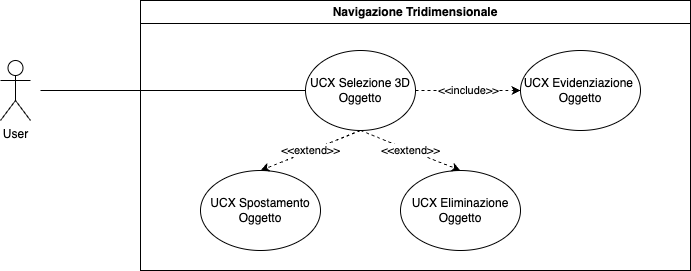
\includegraphics[width=0.8\textwidth]{UseCasesImages/3DSel.png}
%\end{figure}

\vspace{0.5cm}

\large\textbf{} \\
\textbf{Attori:} User\\
\textbf{Pre-condizione:} L'user si trova nell'area di navigazione tridimensionale \\
\textbf{Post-condizione: } Selezione di un oggetto e relativa evidenziazione\\
\textbf{Scenario Principale:}  Navigando nello spazio tridimensionale l'utente seleziona un oggetto che viene conseguentemente evidenziato; una volta selezionato sará possibile spostarlo o eliminarlo.\\
\textbf{Inclusione:} UCX Evidenziazione Oggetto \\
\textbf{Estensioni:} \\ 
-UCX Spostamento Oggetto \\ -UCX Eliminazione Oggetto

\vspace{0.5cm}


\Large\textbf{}\\
\Large\textbf{Use Case X Inserimento Oggetto} \\
%\begin{figure}[h]
% \centering
%  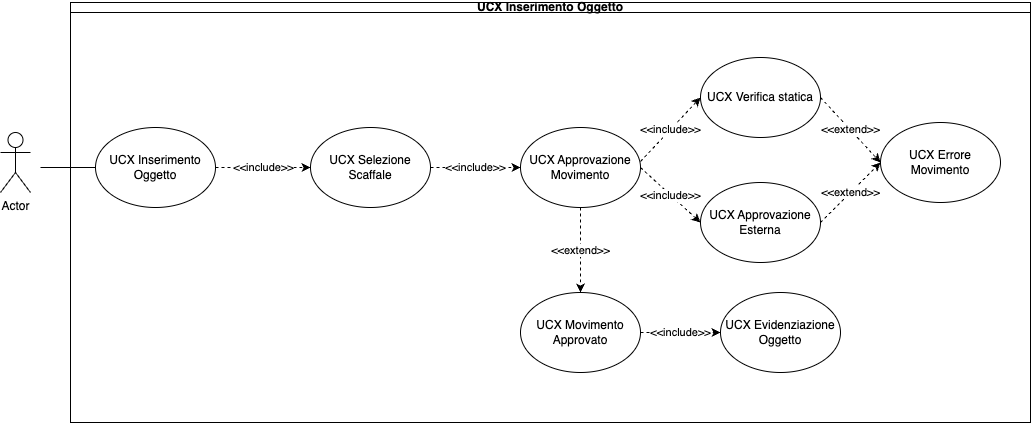
\includegraphics[width=0.8\textwidth]{UseCasesImages/Inserimento.png}
%\end{figure}

\vspace{0.5cm}

\large\textbf{} \\
\textbf{Attori:} User\\
\textbf{Pre-condizione:} L'utente ha selezionato un oggetto  \\
\textbf{Post-condizione: } L'oggetto é stato inserito correttamente oppure viene visualizzato un messaggio di errore\\
\textbf{Scenario Principale:}  Dopo aver selezionato un oggetto l'utente ha scelto di inserirlo nel magazzino, sceglie uno scaffale a cui destinarlo e vengono effettuate una serie di verifiche. La prima verifica effettuata é di natura statica: il sistema verifica la disponibilitá dimensionale del magazzino. Dopo aver passato la verifica statica la richiesta di spostamento viene inoltrata ad un gestore incaricato di approvare il movimento o rifiutarlo. In caso il movimento non venga effettuato viene visualizzato un messaggio di errore \\
\textbf{Inclusione:} UCX Selezione Scaffale \\

\vspace{0.5cm}

\Large\textbf{}\\
\Large\textbf{Use Case X Spostamento Oggetto} \\
%\begin{figure}[h]
%  \centering
%  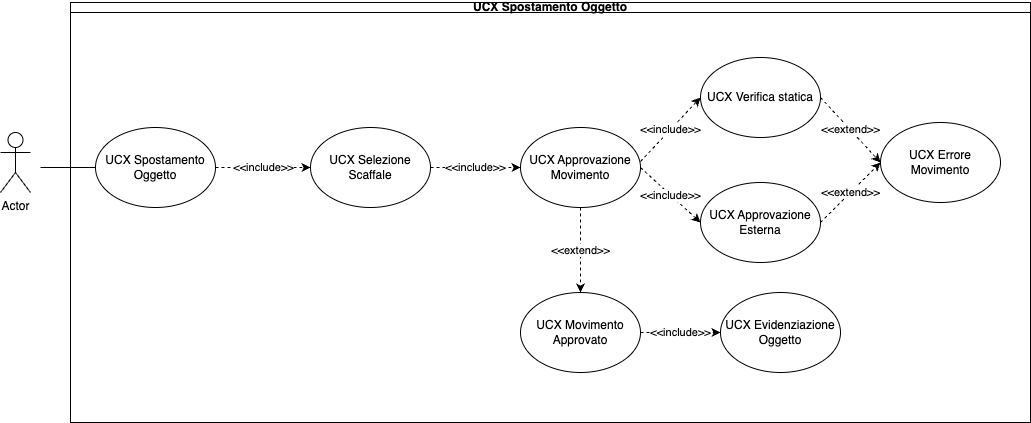
\includegraphics[width=0.8\textwidth]{UseCasesImages/Spostamento.png}
%\end{figure}

\vspace{0.5cm}

\large\textbf{} \\
\textbf{Attori:} User\\
\textbf{Pre-condizione:} L'utente ha selezionato un oggetto  \\
\textbf{Post-condizione: } L'oggetto é stato spostato correttamente oppure viene visualizzato un messaggio di errore\\
\textbf{Scenario Principale:}  Dopo aver selezionato un oggetto l'utente ha scelto di spostarlo, sceglie uno scaffale a cui destinarlo e vengono effettuate una serie di verifiche. La prima verifica effettuata é di natura statica: il sistema verifica la disponibilitá dimensionale del magazzino. Dopo aver passato la verifica statica la richiesta di spostamento viene inoltrata ad un gestore incaricato di approvare il movimento o rifiutarlo. In caso il movimento non venga effettuato viene visualizzato un messaggio di errore \\
\textbf{Inclusione:} UCX Selezione Scaffale \\

\vspace{0.5cm}

\Large\textbf{}\\
\Large\textbf{Use Case X Eliminazione Oggetto} \\

\vspace{0.5cm}

\large\textbf{} \\
\textbf{Attori:} User\\
\textbf{Pre-condizione:} L'utente ha selezionato un oggetto  \\
\textbf{Post-condizione: } L'oggetto é eliminato\\
\textbf{Scenario Principale:}  Dopo aver selezionato un oggetto l'utente ha scelto di eliminarlo \\

\vspace{0.5cm}

\Large\textbf{}\\
\Large\textbf{Use Case X Approvazione Movimento} \\

\vspace{0.5cm}

\large\textbf{} \\
\textbf{Attori:} User\\
\textbf{Pre-condizione:} L'utente ha selezionato un oggetto e uno scaffale a cui destinarlo \\
\textbf{Post-condizione: } Il movimento é stato effettuato correttamente o viene visualizzato un messaggio di errore\\
\textbf{Scenario Principale:} Da Definire \\
\textbf{Inclusione:} \\
UCX Approvazione Statica \\
UCX Approvazione Dinamica \\

\vspace{0.5cm}

\textbf{}\\
{\color{red}{\textbf{Domanda:} Lo spostamento avviene anche attraverso il trascinamento mediante il mouse?}} \\
{\color{red}{\textbf{Delucidamento:} Funzionamento dettagliato della richiesta di approvazione}}\\
\Large\textbf{}\\
\Large\textbf{Use Case 13 - Navigazione nello spazio tridimensionale} \\
\vspace{0.5cm}
\begin{figure}[h]
 \centering
 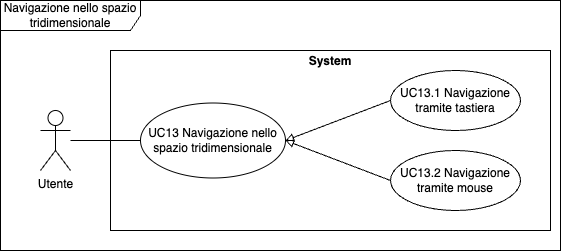
\includegraphics[width=0.8\textwidth]{UseCasesImages/Navigation.png}
\end{figure}
\large\textbf{} \\
\textbf{Attori:} User\\
\textbf{Pre-condizione:} L'utente si trova nello spazio tridimensionale\\
\textbf{Post-condizione: } L'utente ha effettuato un movimento nello spazio tridimensionale\\
\textbf{Scenario Principale:} L'utente effettua un movimento nello spazio tridimensionale attraverso l'utilizzo del mouse o della tastiera\\
\textbf{Generalizzazioni:} 
\begin{itemize}
    \item UC14 Navigazione tramite tastiera
    \item UC15 Navigazione tramite mouse
\end{itemize}
\vspace{0.5cm}

% Struttura dello Use Case - copialo per crearne un altro

%\Large\textbf{}\\
%\Large\textbf{Use Case 1 : Inizializzazione Ambiente} \\
%\vspace{0.5cm}
%\begin{figure}[h]
%  \centering
%  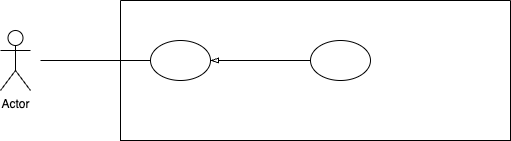
\includegraphics[width=0.8\textwidth]{UseCasesImages/UC1.png}
%\end{figure}

%\large\textbf{} \\
%\textbf{Attori:} \\
%\textbf{Pre-condizione:} \\
%\textbf{Post-condizione:} \\
%\textbf{Scenario Principale:} \\
%\textbf{Generalizzazioni:} \\

%\vspace{0.5cm}

% Fine use case

\section{REQUISITI}\label{sec:requisiti}
La seguente sezione si occupa di \textbf{Descrivere}, \textbf{Classificare}, \textbf{Tracciare} e \textbf{Codificare}
i requisiti individuati dal gruppo. \\
Una prima macrodivisione classificativa sarà effettuata tra requisiti:
\begin{itemize}
    \item \textbf{Funzionali: }indicano le funzionalità offerta all'utente
    \item \textbf{di Interfaccia: }indicano i requisiti offerti dall'interfaccia
    \item \textbf{di Database: }indicano i requisiti di interazione con la base di dati
    \item \textbf{Di Qualità: } garantiscono la qualità del prodotto
    \item \textbf{Di Sistema: }indicano le specifiche tecniche a supporto dell'utiluzzo del prodotto
   % \item \textbf{Di Vincolo: } indicano i vincoli logici del sistema
\end{itemize}
i quali meritano una suddivisione in sottosezioni apposite.\\
Ci si occuperà inoltre di distinguerà tra requisiti \textbf{Obbligatori}, \textbf{Desiderabili} ed \textbf{Opzionali}.\\ 
Di particolare importanza è inoltre il tracciamento dell'origine dei requisiti, in cui si esamina il perimetro di origine dei tali: una prima suddivisione sará effettuata tra requisiti \textbf{espliciti} ed \textbf{impliciti}, a cui sarà aggiunta una citazione del documento o la modalità dalla quale lo si è ricavatot, con eventuali riferimenti ai Casi d'uso individuati nella prima parte di questo docuemnto.\\
Sulla base delle specifiche appena discusse, ad ogni documento verrà assegnato un codice che segue la seguente regola:

\begin{figure}[h]
 \centering
  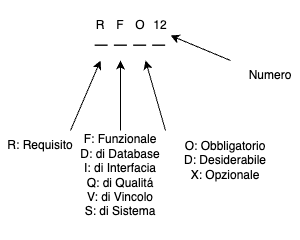
\includegraphics[width=0.5\textwidth]{UseCasesImages/requirementsCod.png}
\end{figure}

\subsection{Requisiti funzionali}

\setlength{\arrayrulewidth}{0.5mm}
\renewcommand{\arraystretch}{2.5}

\begin{table}[h]
\centering
\rowcolors{3}{gray!10!white!100}{gray!0!white!100}
\begin{tabular}{ |>{\centering\arraybackslash}p{1cm}|>{\centering\arraybackslash}p{9cm}|>{\centering\arraybackslash}p{5cm}| }
\hline
\multicolumn{3}{|c|}{\Large Requisiti funzionali} \\
\hline
Codice & Descrizione & Tracciamento\\
\hline
RFD1 & L'utente può caricare un file per inizializzare l'ambiente& Esplicito, Capitolato\\
RFO1 & L'utente può creare un ambiente da zero & Esplicito, Capitolato \\
RFO2 & L'utente può creare delle scaffalature & Esplicito, Capitolato\\
RFO3 & L'utente può creare un oggetto & Esplicito, Capitolato\\
RFO4 & L'utente può navigare nello spazio tridimensionale attraverso il mouse& Esplicito, Capitolato\\
RFO5 & L'utente può navigare nello spazio tridimensionale attraverso la tastiera& Esplicito, Capitolato\\
RFO6 & L'utente può scegliere la dimensione delle scaffalature & Implicito, Analisi dei requisiti\\
RFO7 & L'utente può modificare le scaffalature create & Esplicito, Capitolato\\
\hline
\end{tabular}
\end{table}

\newpage

\begin{table}[h]
\centering
\rowcolors{3}{gray!10!white!100}{gray!0!white!100}
\begin{tabular}{ |>{\centering\arraybackslash}p{1cm}|>{\centering\arraybackslash}p{9cm}|>{\centering\arraybackslash}p{5cm}| }
\hline
\multicolumn{3}{|c|}{\Large Requisiti funzionali} \\
\hline
Codice & Descrizione & Tracciamento\\
\hline
RFO8 & L'utente può eliminare le scaffalature create & Implicito, Analisi dei requisiti\\
RFO8 & L'utente può eliminare un oggetto creato & Implicito, Analisi dei requisiti\\
RFO9 & L'utente può selezionare una scaffalatura nello spazio tridimensionale & Esplicito, Capitolato\\
RFO10 & L'utente può selezionare un oggetto nello spazio tridimensionale & Esplicito, Capitolato\\
RFD2 & L'utente può ricercare un oggetto tramite id & Esplicito, Capitolato\\
RFO11 & L'utente può inserire un oggetto all'interno di una scaffalatura& Esplicito, Capitolato\\
RFO12 & L'utente può richiedere lo spostamento di un oggetto & Esplicito, Capitolato\\
RFO13 & L'utente può rimuovere un oggetto da una scaffalatura & Implicito, Analisi dei requisiti\\
RFO14 & Il sistema deve verificare la disponibilità della scaffalatura target alla richiesta di uno spostamento & Implicito, Dialogo con il Proponente\\
RFO14 & Il sistema delega ad un meccanismo terzo la decisione finale sull'accettazione di un movimento & Implicito, Dialogo con il Proponente\\
\hline
\end{tabular}
\end{table}



\subsection{Requisiti di Interfaccia}

\setlength{\arrayrulewidth}{0.5mm}
\renewcommand{\arraystretch}{2.5}

\begin{table}[h]
\centering
\rowcolors{3}{gray!10!white!100}{gray!0!white!100}
\begin{tabular}{ |>{\centering\arraybackslash}p{1cm}|>{\centering\arraybackslash}p{9cm}|>{\centering\arraybackslash}p{5cm}| }
\hline
\multicolumn{3}{|c|}{\Large Requisiti di Interfaccia} \\
\hline
Codice & Descrizione & Tracciamento\\
\hline
RID1 & L'utente può scegliere come inizializzare il suo ambiente & Esplicito, Capitolato\\
RIO1 & Sviluppo di un'are gestionale nella quale effettuare le ricerche per Id & Implicito, Analisi dei Requisiti\\
RIX1 & Un oggetto selezionato viene evidenziato nell'ambiente tridimensionale & Esplicito, Capitolato\\
\hline
\end{tabular}
\end{table}

\newpage

\subsection{Requisiti di Database}

\setlength{\arrayrulewidth}{0.5mm}
\renewcommand{\arraystretch}{2.5}

\begin{table}[h]
\centering
\rowcolors{3}{gray!10!white!100}{gray!0!white!100}
\begin{tabular}{ |>{\centering\arraybackslash}p{1cm}|>{\centering\arraybackslash}p{9cm}|>{\centering\arraybackslash}p{5cm}| }
\hline
\multicolumn{3}{|c|}{\Large Requisiti di Database} \\
\hline
Codice & Descrizione & Tracciamento\\
\hline
RDO1 & Il Database deve memorizzare le scaffalatura tramite coordinate&Esplicito, Capitolato\\
RDD1 & Il Database deve memorizzare la posizione degli oggetti ed il loro nome & Implicito, Analisi dei Requisiti\\
\hline
\end{tabular}
\end{table}
\newpage

\subsection{Requisiti di Qualità}

\setlength{\arrayrulewidth}{0.5mm}
\renewcommand{\arraystretch}{2.5}

\begin{table}[h]
\centering
\rowcolors{3}{gray!10!white!100}{gray!0!white!100}
\begin{tabular}{ |>{\centering\arraybackslash}p{1cm}|>{\centering\arraybackslash}p{9cm}|>{\centering\arraybackslash}p{5cm}| }
\hline
\multicolumn{3}{|c|}{\Large Requisiti di Qualità} \\
\hline
Codice & Descrizione & Tracciamento\\
\hline
\hline
\end{tabular}
\end{table}
\newpage

\subsection{Requisiti di Sistema}

\setlength{\arrayrulewidth}{0.5mm}
\renewcommand{\arraystretch}{2.5}

\begin{table}[h]
\centering
\rowcolors{3}{gray!10!white!100}{gray!0!white!100}
\begin{tabular}{ |>{\centering\arraybackslash}p{1cm}|>{\centering\arraybackslash}p{9cm}|>{\centering\arraybackslash}p{5cm}| }
\hline
\multicolumn{3}{|c|}{\Large Requisiti di Sistema} \\
\hline
Codice & Descrizione & Tracciamento\\
\hline
\hline
\end{tabular}
\end{table}

\section{Riepilogo}
Di seguito si propone una suddivisione dei requisiti per rilevanza, conteggiandone il numero:

\begin{center}
\begin{tabular}{ c c c c }
 Obbligatori & Desiderabili & Opzionali & Totale \\ 
 17 & 4 & 1 & \textcolor{red}{23}
\end{tabular}
\end{center}